\documentclass[12pt,a4paper]{article}

\usepackage[left=2cm,right=2cm,top=2cm,bottom=2cm]{geometry} % less blank area
\usepackage{amsmath,amssymb,bm,dsfont} % for math
\usepackage{array}   % for eqnarray
\usepackage{arydshln}
\usepackage{graphicx}
\usepackage{enumerate} % for stylish enumrate
\usepackage{listings} % for code demonstration
\usepackage{color}    % for code highlight
\usepackage{fancyhdr} % for header and footnote
\usepackage{lastpage} % for calculating total pages
\usepackage{subfig} % for subfigure
\usepackage{tikz} % for drawing
\usepackage{pdfpages} % for importing PDF files

\newcommand{\docTitle}{IN2106 Practical Course -- Vision-based Navigation: Exercise \#4}
\newcommand{\docSubtitle}{Topic: Visual Odometry}
\newcommand{\docAuthor}{Min-An Chao (03681062)}
\newcommand{\docAuthorDept}{TUM MS Informatics}
\newcommand{\docAuthorEmail}{ga83fok@mytum.de}
\newcommand{\docDate}{24.05.2018}

\pagestyle{fancy}
\fancyhf{}
\lhead{\textit{\docTitle}}
\rhead{\textit{\docAuthor}}
\cfoot{\textit{- Page \thepage of \pageref{LastPage} -}}

\lstset{ language={},
         basicstyle=\ttfamily\footnotesize,
         keywordstyle=\color{blue}\ttfamily\footnotesize,
         commentstyle=\color{magenta}\ttfamily\footnotesize,
         morecomment=[l][\color{magenta}\footnotesize]{\#}
}

\setlength{\parindent}{0cm}
\setlength{\parskip}{0.5cm}

% for vector and matrix
\newcommand{\vct}[1]{\boldsymbol{#1}}
\newcommand{\mtx}[1]{\mathbf{#1}}
\newcommand{\set}[1]{\mathcal{#1}}
\newcommand{\dom}[1]{\mathbb{#1}}
\newcommand{\fnc}[1]{\text{#1}}

\DeclareMathOperator*{\argmin}{argmin}
\DeclareMathOperator*{\argmax}{argmax}

% for alignment argument of matrix/pmatrix
\makeatletter
\renewcommand*\env@matrix[1][c]{\hskip -\arraycolsep
  \let\@ifnextchar\new@ifnextchar
  \array{*\c@MaxMatrixCols #1}}
\makeatother

\begin{document}
    \title{\vspace{-1.75cm} \large \textsf{\textbf{\docTitle}}\\ \textsf{\docSubtitle}}
    \author{\normalsize \textsf{
        \textbf{\docAuthor} \hspace{6pt}\textbar\hspace{6pt}
        \docAuthorDept \hspace{6pt}\textbar\hspace{6pt}
        \docAuthorEmail}}
    \date{\small \textsf{\docDate}}
    \maketitle 
    \thispagestyle{fancy}
    \vspace{-0.5cm}
    \hrule
    
    \section{Feature based visual odometry}
    \textsf{\textbf{Task 1}}
    The feature points are labeled with angles,
    as shown in Fig.~\ref{fig:feat1}.
    The \texttt{atan()} function is used
    to compute the angle,
    along with wrap-around check for negative $m_{10}$
    and radius-to-degree conversion.
    (\texttt{OpenCV} use degree as unit for plotting.)
    
    \begin{figure}[!h]
        \centering
        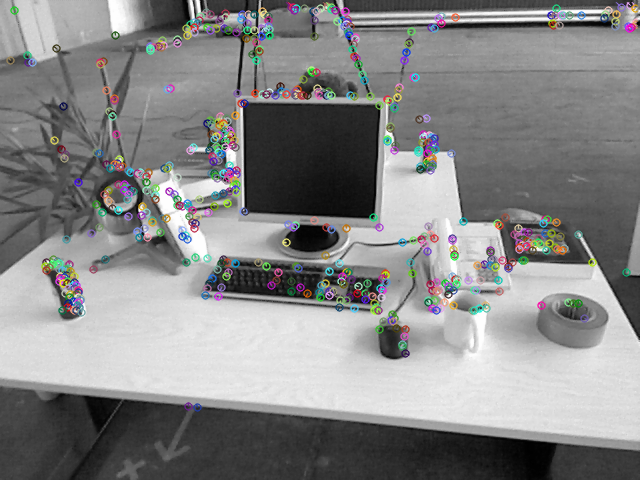
\includegraphics[height=6cm]{fig/feat1.png}
        \caption{Feature points with angles labeled}
        \label{fig:feat1}
    \end{figure}
    
    \textsf{\textbf{Task 2}}
    Based on the rotation angle of each feature point,
    we compute the rotated point based on the sample points
    given by \texttt{ORB\_pattern}.
    The rotated points outside the image will be marked as 
    "bad" points, and below shows the number of such
    bad points.
    Other good points, 
    where we use to get the pixel values in two images,
    will come up of a corresponding Boolean value,
    labeling if pixel from image 1 is larger than another.
    \begin{lstlisting}[frame=single,numbers=left]
bad/total: 41/638
bad/total: 6/595
    \end{lstlisting}
    
    \textsf{\textbf{Task 3}}
    By computing the nearest point in image 2 for each point in image 1,
    we obtain a vector matches stored as \texttt{matches}
    with data type \texttt{vector<cv::DMatch>}.
    However, there will be some 2 or more matches in the vector \texttt{matches},
    that share the same point in image 2 as the nearest point.
    We can mark such matches as conflicts.
    Since the matches should be exclusively one-to-one in 2 images,
    we delete all such conflicts inside the vector \texttt{matches}.
    After this we obtain what we expected, as shown in Fig.~\ref{fig:matches}.
    
    \begin{figure}[!h]
        \centering
        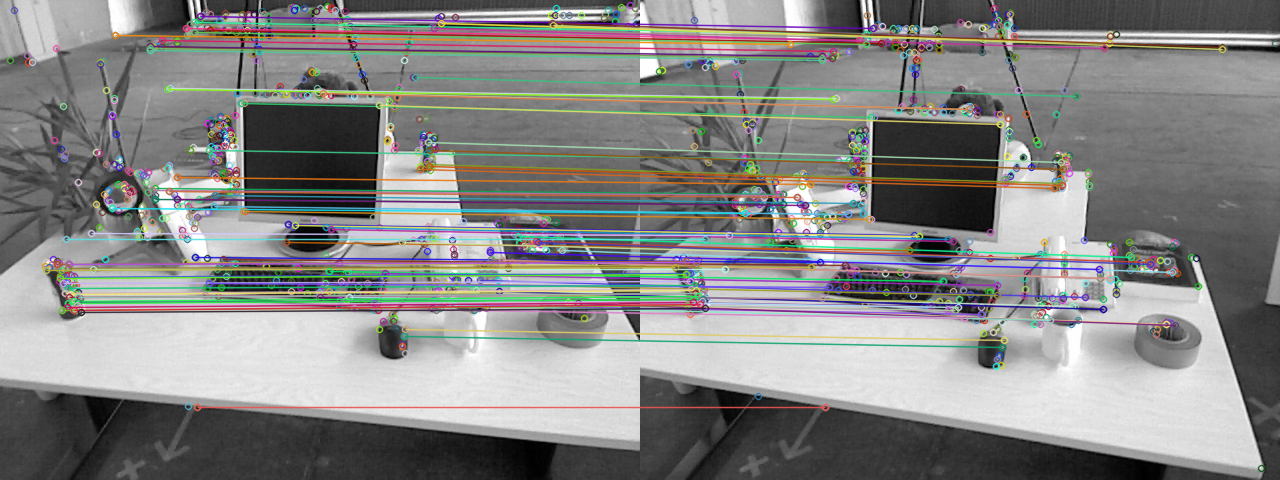
\includegraphics[height=6cm]{fig/matches.png}
        \caption{Matches made by brute force searching from feature points}
        \label{fig:matches}
    \end{figure}

    \textsf{\textbf{Task 4}}
    2D-2D pose estimation can be done by \texttt{OpenCV} functions
    \texttt{findEssentialMat()} and \texttt{recoverPose()}.
    The results are shown below.
    \begin{lstlisting}[frame=single,numbers=left]
essential_matrix is 
[-0.01689316757952954, -0.4001360984609538, -0.05206126359774105;
 0.382602780486801, -0.03388384497843067, 0.5922787440926547;
 0.0145439817260907, -0.5814930982650205, -0.0149159111406146]
estimated motion using 2D-2D method
Rotation from 1 to 2: 
  0.998461 -0.0461534   0.030742
 0.0453012   0.998585  0.0278645
-0.0319845 -0.0264289   0.999139
translation from 1 to 2: 
 -0.820848 -0.0578427   0.568211
    \end{lstlisting}

    After processing depth information from RGB-D camera,
    we obtain the 3D information of keypoints,
    where $(u,v)$ is transformed to $(x,y)$ coordinate
    and then applied with depth information to be
    $(x',y',z') = (xd, yd, d)$.
    With \texttt{OpenCV} functions
    \texttt{solvePnP()} and \texttt{Rodrigues()}.
    The results are shown below.
    Note the rotation matrix is similar to 2D-2D result,
    with translation only scaled down compared to 2D-2D.
    \begin{lstlisting}[frame=single,numbers=left]
estimated motion using 3D-2D method
Rotation from 1 to 2: 
  0.998263 -0.0504054  0.0304982
   0.04982   0.998565  0.0196607
-0.0314454 -0.0181071   0.999341
translation from 1 to 2: 
  -0.11344 0.00391171  0.0685656
    \end{lstlisting}

    Finally, we transform keypoints from both image 1 and 2
    with the same procedures to obtain their 3D information.
    Subtracted with mass center $\vct{\bar{p}}_1$ and $\vct{\bar{p}}_2$ for each array,
    we have $\vct{q}_1^{(i)}$ and $\vct{q}_2^{(i)}$, and
    we compute $\mtx{W} = \sum_i \vct{q}_1^{(i)} {\vct{q}_2^{(i)}}^T$.
    Then by SVD decomposition of $\mtx{W} = \mtx{US}\mtx{V}^T$,
    we get rotation $\mtx{R} = \mtx{U}\mtx{V}^T$
    and $\vct{t} = \vct{\bar{p}}_1 - \mtx{R}\vct{\bar{p}}_2$.
    The results are shown below.
    Perhaps due to the noise in depth information, 
    the results do not look so similar.
    \begin{lstlisting}[frame=single,numbers=left]
estimated motion using 3D-3D method
Rotation from 1 to 2: 
  0.995954  0.0787748 -0.0432516
-0.0707982   0.984202   0.162275
 0.0553515  -0.158556   0.985797
translation from 1 to 2: 
 0.116904 -0.289467 0.0741315
    \end{lstlisting}

    \section{LK optical flow}
    
    \textsf{\textbf{Task 1}}
    The Jacobian matrix is derived from error related to the motion as
    \begin{eqnarray}\label{eq:lk_fwd}
      \vct{J}_i = \begin{pmatrix}
        -\frac{\partial I_2(x_i + \Delta x_i, y_i + \Delta y_i)}{\partial x_i} &
        -\frac{\partial I_2(x_i + \Delta x_i, y_i + \Delta y_i)}{\partial y_i} 
      \end{pmatrix}^T,
    \end{eqnarray}
    along with 
    \begin{eqnarray}
      \mtx{H} &=& \sum_i \vct{J}_{i} \vct{J}_{i}^T, \nonumber\\
      \vct{b} &=& \sum_i - e_i \vct{J}_{i} , \nonumber\\
      (\partial x_i, \partial y_i)^T &=& \mtx{H}^{-1} \vct{b}. 
    \end{eqnarray}
    
    \textsf{\textbf{Task 2}}
    We change the optimization object in Eq.~\ref{eq:lk_fwd}
    to derive an inverse version:
    \begin{eqnarray}\label{eq:lk_inv}
      \vct{J}_i = \begin{pmatrix}
        -\frac{\partial I_1(x_i , y_i)}{\partial x_i} &
        -\frac{\partial I_1(x_i , y_i)}{\partial y_i} 
      \end{pmatrix}^T.
    \end{eqnarray}
    The result of single layer optical flow is shown in Fig.~\ref{fig:lkflow_single}.
    
    \begin{figure}[!h]
        \centering
        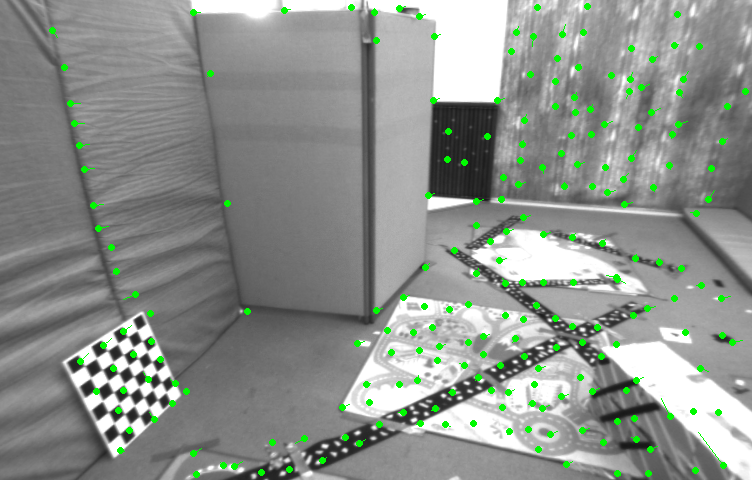
\includegraphics[height=6cm]{fig/LKflow_single.png}
        \caption{LK flow using single layer}
        \label{fig:lkflow_single}
    \end{figure}
    
    \textsf{\textbf{Task 3}}
    In multi-layer method,
    coarse-to-fine means we downsample the original image to get a coarse optical flow first,
    then upsample back the candidates to gradually refine our optical flow estimates.
    The pyramid method used in pixel level or feature point level is basically the same.
    Only the projection needs to be done if feature points are stored in 3D world coordinate.
    
    The results are in Fig.~\ref{fig:lkflow_multi},
    with multi-layer LK flow slightly better than \texttt{OpenCV} implementation.

    \begin{figure}[!ht]
        \centering
        \subfloat[multi-layer LK]{
            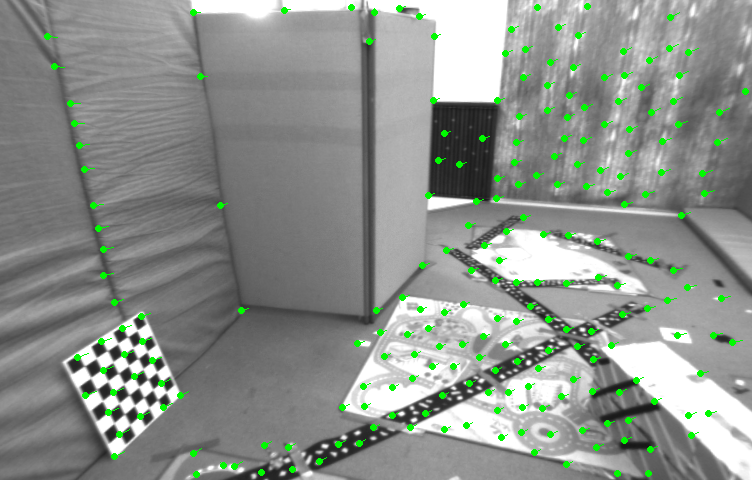
\includegraphics[height=5cm]{fig/LKflow_multi.png}
        }
        \subfloat[\texttt{OpenCV} library]{
            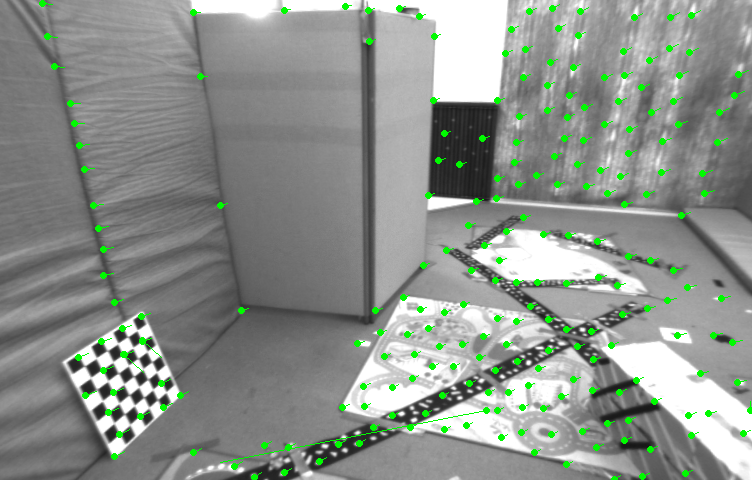
\includegraphics[height=5cm]{fig/LKflow_opencv.png}
        }
        \caption{LK flow results}
        \label{fig:lkflow_multi}
    \end{figure}

    \section{Direct method}
    
    \textsf{\textbf{Task 1}}
    The $6 \times 1$ Jacobian matrix can be factorizes as two part,
    the 3D-2D projection part $2 \times 6$ $\mtx{J}_{\xi}$,
    and the image pixel gradient part $2 \times 1$ $\mtx{J}_{p}$.
    \begin{eqnarray}\label{eq:lk_fwd}
      \mtx{J}_i &=& \mtx{J}_{\xi,i}^T \mtx{J}_{p,i}, \nonumber\\
      \mtx{J}_{\xi,i} &=& \begin{pmatrix}
        -\frac{f_x}{z_{i}} & 0 & \frac{f_x  x_{i}}{z_{i}^2} & \frac{f_x  x_{i} y_{i}}{z_{i}^2} & -f_x - \frac{f_x  x_{i}^2}{z_{i}^2} & \frac{f_x y_{i}}{z_{i}} \\
        0 & -\frac{f_y}{z_{i}} & \frac{f_y  y_{i}}{z_{i}^2} & f_y + \frac{f_y  y_{i}^2}{z_{i}^2} & -\frac{f_y x_{i} y_{i}}{z_{i}^2} & -\frac{f_y x_{i}}{z_{i}} 
      \end{pmatrix}, \nonumber\\
      \mtx{J}_{p,i} &=& \begin{pmatrix}
        \frac{\partial I_{\text{cur}}(u_i , v_i)}{\partial u_i} &
        \frac{\partial I_{\text{cur}}(u_i , v_i)}{\partial v_i} 
      \end{pmatrix}^T, \nonumber\\
      \text{where } (u_i,v_i) &=&
      (\frac{x_i}{z_i}\cdot f_x + c_x, \frac{y_i}{z_i}\cdot f_y + c_y).
    \end{eqnarray}
    
    The size of window, or patch, is chosen to be $4 \times 4$ in this task.
    However it also makes sense to just choose a single pixel,
    just with weaker ability to fight against noise and sudden illumination changes.
    
    \textsf{\textbf{Task 2}}
    The results are shown with trajectories of sample points in Fig.~\ref{fig:direct}
    for each frame. The pose shift portions from the first to the fifth
    image are shown as follows.
    \begin{lstlisting}[frame=single,numbers=left]
t1 = (-0.00153993, 0.00281099, -0.72449)^T
t2 = (0.0072663, -0.00159868, -1.47007)^T
t3 = (0.00767712, 0.00385026, -2.20899)^T
t4 = (0.010734, 0.00301489, -2.99649)^T
t5 = (0.0171474, -0.00840279, -3.78821)^T
    \end{lstlisting}

    \begin{figure}[!ht]
        \centering
        \subfloat[Reference]{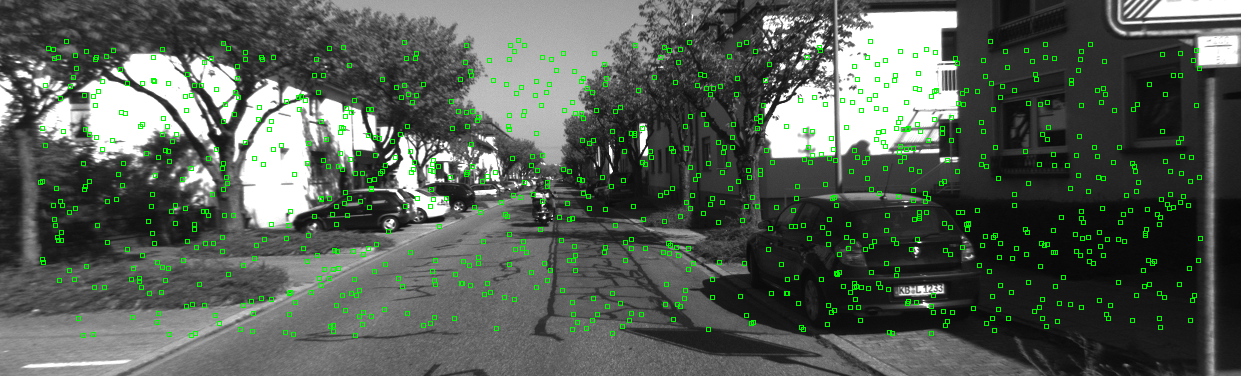
\includegraphics[height=3cm]{fig/direct_reference.png}} \vfill
        \subfloat[Current-1]{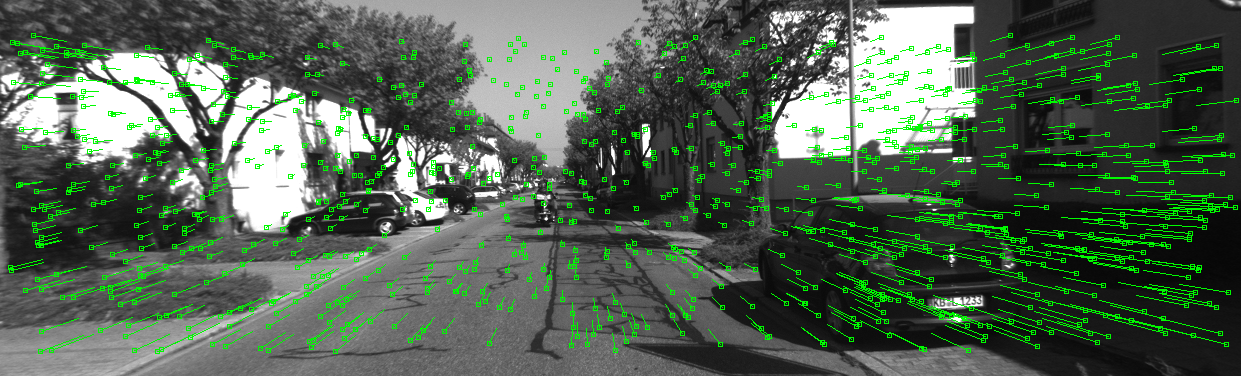
\includegraphics[height=3cm]{fig/direct_current1.png}}\vfill
        \subfloat[Current-2]{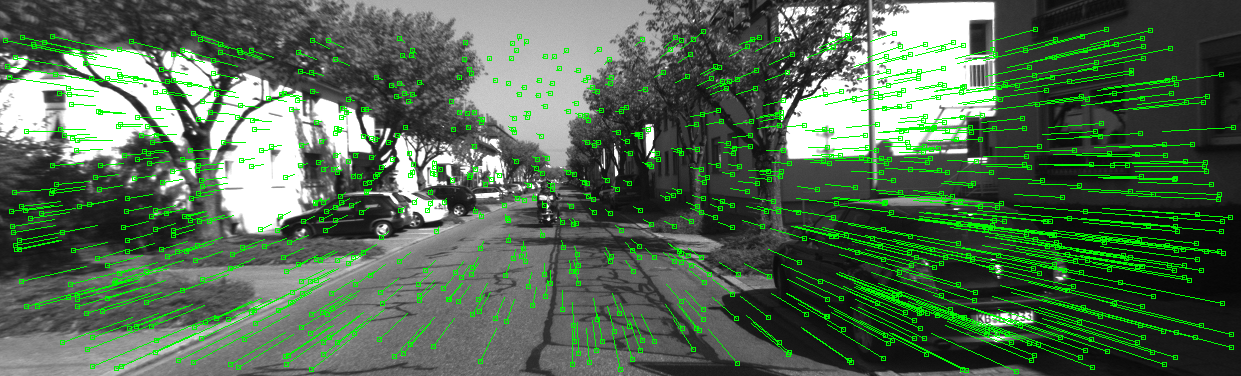
\includegraphics[height=3cm]{fig/direct_current2.png}}\vfill
        \subfloat[Current-3]{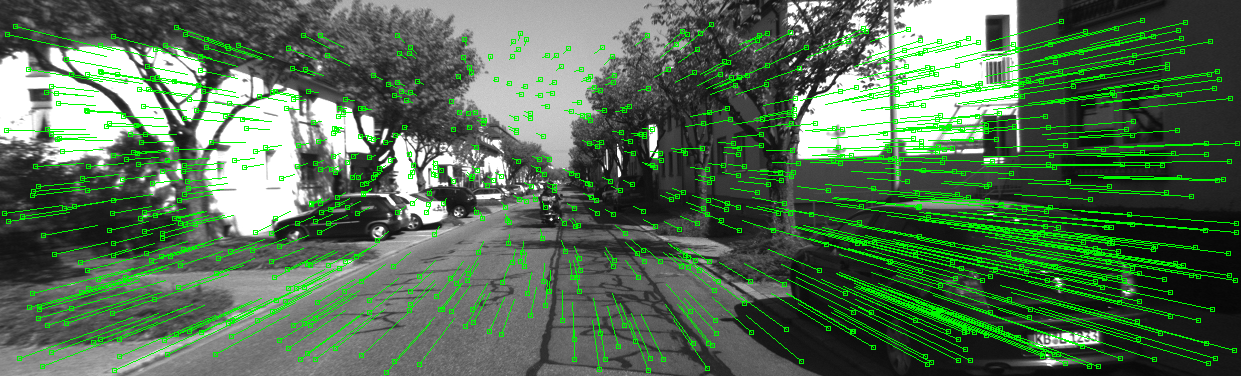
\includegraphics[height=3cm]{fig/direct_current3.png}}\vfill
        \subfloat[Current-4]{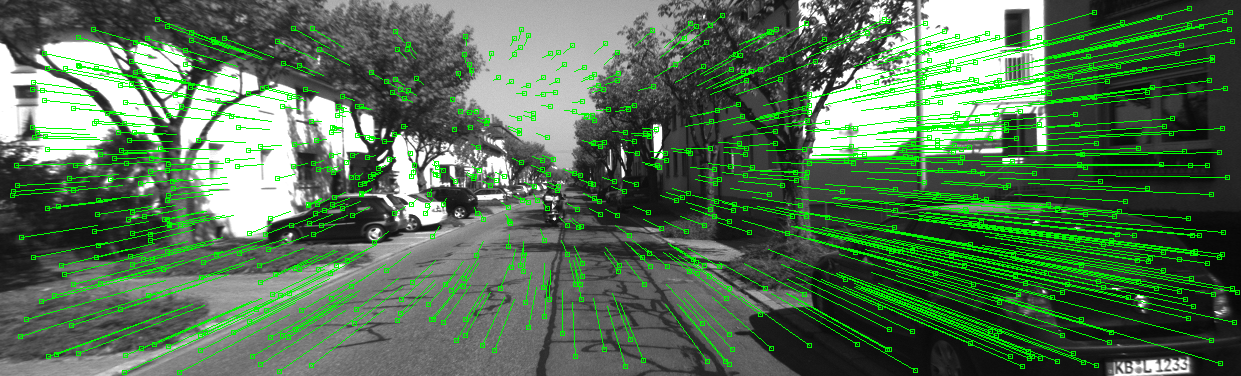
\includegraphics[height=3cm]{fig/direct_current4.png}}\vfill
        \subfloat[Current-5]{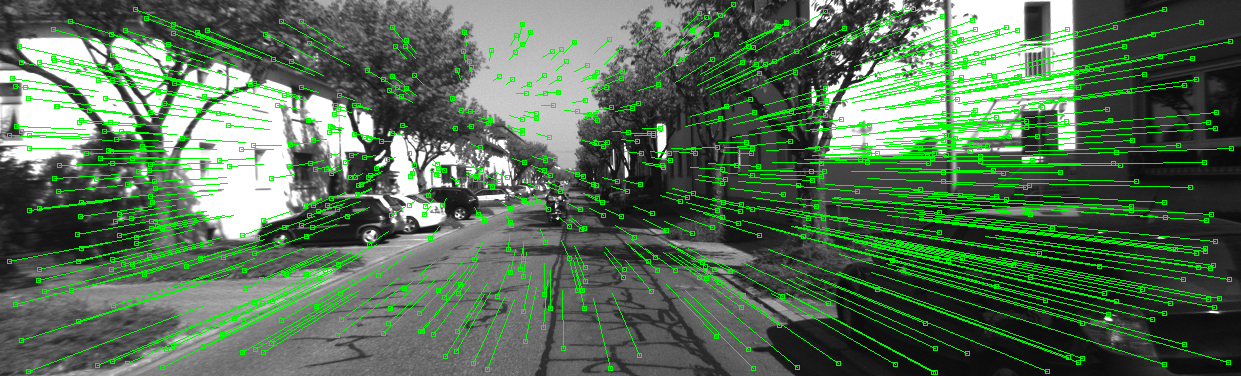
\includegraphics[height=3cm]{fig/direct_current5.png}}
        \caption{Results of direct method}
        \label{fig:direct}
    \end{figure}

    \textsf{\textbf{Task 3}}

    We can use the similar concepts of inverse and compositional method
    from optical flow as well
    since we compute directly based on pixel points.
    The computation $\mtx{J}_{\xi}$ is invariant to the patch,
    thus should be cached for all pixels in a patch.
    Since we use 3D-2D projection to obtain possible pixel value of a point,
    there is no necessary to be some points with strong features like corners.
    So direct method could be useful for sequences lack of feature points,
    or images that features are difficult to extracted,
    and provides fast tracking ability.
    However its weak spot would be the cases like sudden change of movement
    or illumination between 2 frames.

%% template for figures
%   \begin{figure}[!h]
%       \centering
%       \includegraphics[height=6cm]{fig/xxx.png}
%       \caption{XXX}
%       \label{fig:xxx}
%   \end{figure}
%% template for source code or results
%   \begin{lstlisting}[frame=single,numbers=left]
%   \end{lstlisting}
    
\end{document}
